
\documentclass{article}
\usepackage{amsmath}
\usepackage{graphicx}
\usepackage{amssymb}

\title{Probability}
\author{Keith Goh}
\begin{document}
\maketitle

\section{W1C1}
Permutation
$$
nx(n-1)x...x(n-k+1)=\frac{n!}{n-k!}=:P^n_k
$$
This is the number of ways to choose and arrange k distinct objects from n distinct objects(order of picking matters)This is because we want them to fill up some unique positions\\
permutation without repetition if there are identical objects then we must divide by the number of  identical factorial
$$
\frac{n!}{n_1!n_2!....n_r!}
$$
where $n_r$  is the number of identical objects \\
If order does not matter when we pick our objects then we use
$$
{n \choose k} = C^n_k=\frac{P^n_k}{k!}=\frac{n!}{k!(n-k)!}
$$
Remember the slotting method when you are arranging objects such that no 2 of a type are beside each other.\\
divide n distinct objects into r diff piles of size n1,n2
$$
{n \choose n_1}{n-n_1 \choose n_2}=\frac{n!}{n_1!n_2!...n_r!}
$$
\section{w1c2}
$$
(a+b)^n=\sum_{k=0}^n{n \choose k}a^kb^{n-k}
$$
counting given n distinct objects find the arrangements of k of them where order does not matter but repetitions are allowed\\
Multichoose
$$
{k+n-1 \choose n-1}
$$
n-1 is number of bars\\
we can think of it as having k+n-1 objects and n-1 will transform into the bars.\\
Circular symmetry
$$
\frac{n!}{n}
$$
\begin{enumerate}
  \item Remember when counting 2 separate cases make sure they are unique before adding unless minus the intersection
  \item Check complements sometimes, its easier to do
  \item when you splitting into equal unlabeled piles rmb to divide by n!, n being the number of piles after doing choosing.
  \item alternative general formula $\frac{n!}{h!^kk!}$
\end{enumerate}
Extra:\\
Multinomial Theorem
$$
(x_1+x_2+x_3...x_k)^n=\sum_{B_1+b_2...b_k=n}{n \choose b_1,b_2,b_3,....b_k}\prod_{j=1}^kx^{b_j}_j
$$
\section{w2c1}
Axioms of probability
\begin{enumerate}
  \item 0$\leq P(E)\leq 1$
  \item P(S)=1
  \item $P(\bigcup_{i=1}^{\infty}E_i)=\sum_{i=1}^{\infty}P(E_i)$
\end{enumerate}
Axiom 3 finite version\\
$$
\mathbb{P}(\bigcup_{i=1}^{n}E_i)=\sum_{i=1}^n\mathbb{P}{E_i}
$$
inclusion exclusion
$$
\mathbb{P}(A \cup B)=\mathbb{P}A+\mathbb{P}B-\mathbb{P}{A\cap B}
$$
$$
\mathbb{P}(A\cup B \cup C )=\mathbb{P}(A)+\mathbb{P}(B)+P(C)-\mathbb{P}(A\cap B)- \mathbb{P}(B\cap C)-\mathbb{P}(C\cap A)+\mathbb{P}(A\cap B \cap C)
$$
\section{W2C2}
Hypergeometric distribution\\
$$
\mathbb {P}(\text{r men on a committee of k people})=\frac{{n \choose r}{m \choose k-r}}{{n+m \choose k}}
$$
Arithmetic Series
$$
1+2+3+...+n=\frac{n(n+1)}{2}
$$
Taylor Series for $e^x$
$$
\sum_{n=0}^{\infty}\frac{x^n}{n!}=e^x
$$
Geometric Series
$$
1+r+r^2+...+r^{n-1}=\frac{1-r^n}{1-r}
$$

if $|r|<$1 and $n\rightarrow \infty$,
$$
1+r+r^2+...=\frac{1}{1-r}
$$
$$
P(d,n)=1-(1-\frac{1}{d})(1-\frac{2}{d})....(1-\frac{n-1}{d})
$$
this equations to
$$
P(d,n)\approx 1-e^{1/d}e^{-2/d}....e^{-(n-1)/d}
$$
when using the identity $e^{-x}\approx 1-x$
Derangement
$$
D_n=n!(1-\frac{1}{1!}+\frac{1}{2!}-\frac{1}{3!}+...+(-1)^n\frac{1}{n!})
$$
$$
D_n=(n-1)(D_{n-1}+D_{n-2})
$$
\section{w3C1}
Definition(conditional Probability)\\
if P(B)$>$0, then
$$
\mathbb{P}(A|B):=\frac{\mathbb{P}{(A \cap B)}}{\mathbb{P}(B)}
$$
hence
$$
\mathbb{P}(A \cap B)=\mathbb{P}(B)\mathbb{P}(A|B)=\mathbb{P}(A)\mathbb{P}(B|A)
$$
which allows us to multiply probabilities \\
interesting result which is proven from the definition of conditional probability\\
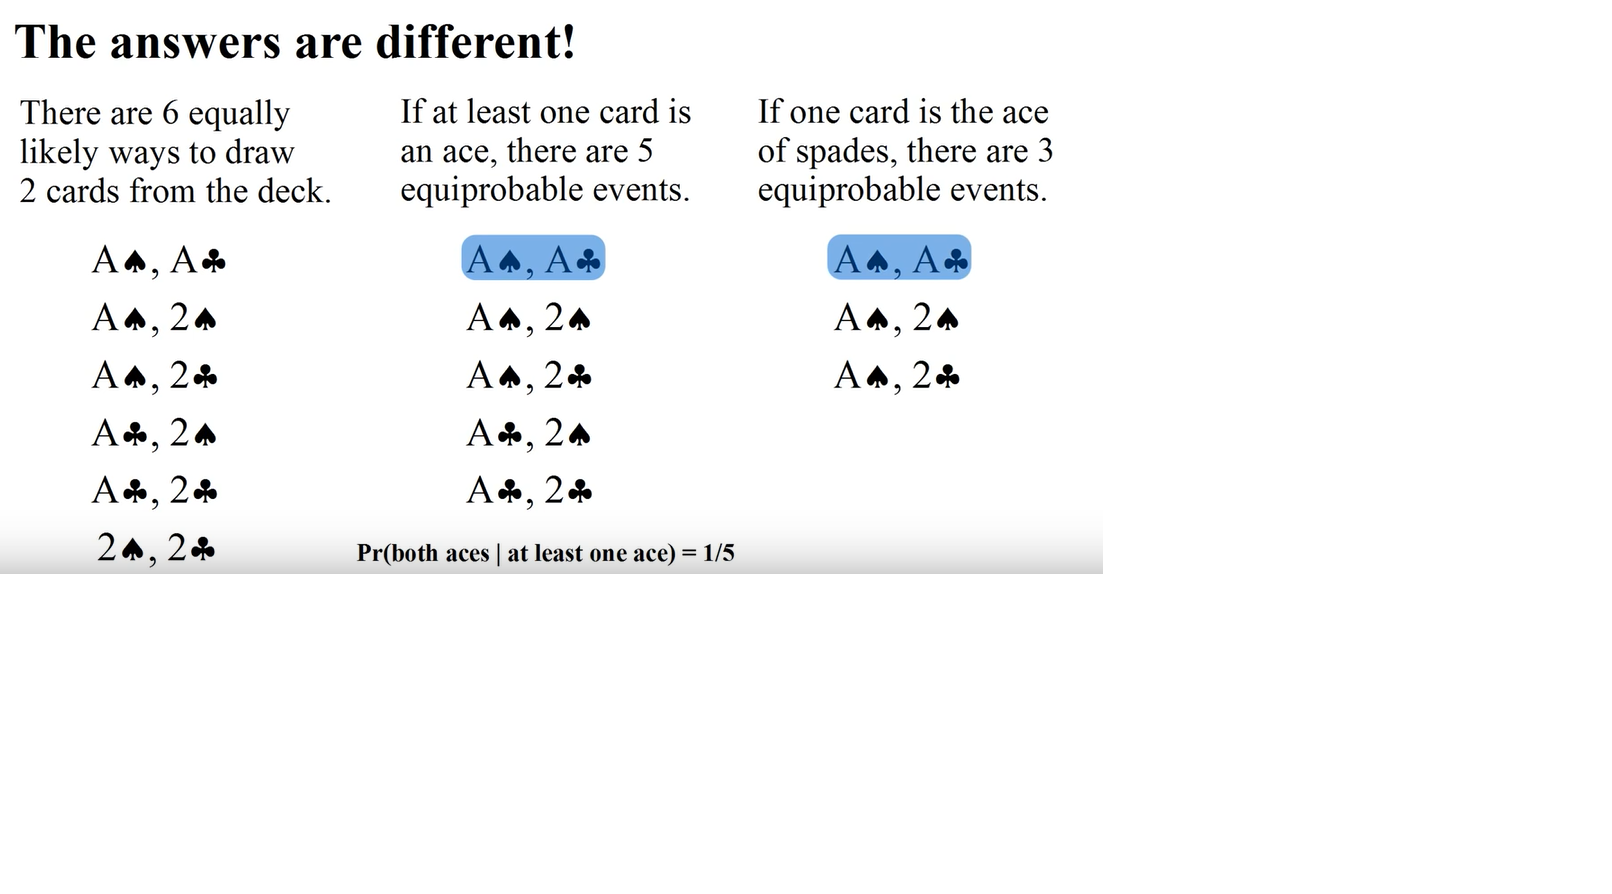
\includegraphics[width=\textwidth]{different}
Law of total probability
$$
\mathbb{P}(A)=\mathbb{P}(B_1)\mathbb{P}(A|B_1)+\mathbb{P}(B_2)\mathbb{P}(A|B_2)+...+\mathbb{P}(B_n)\mathbb{P}(A|B_n)
$$
\section {W3C2}
Bayes' Law(Bae's)
$$
\mathbb{P}(A|B)=\frac{\mathbb{P}{(B|A)}\mathbb{P}{(A)}}{\mathbb{P}(B)}
$$
where
$$
\mathbb{P}{(B)}=\mathbb{P}(B|A)\mathbb{P}(A)+\mathbb{P}(B|A^c)\mathbb{P}A^c
A|A$$
Independent
$$
\mathbb{P}(A|B)=\mathbb P (A)
$$
$$
\mathbb P (B|A)=\mathbb P (B)
$$
$$
\mathbb P (A\cap B)=\mathbb P (A) \mathbb P (B)
$$
Three events are independent if they are pairwise independent and
$$
\mathbb P (A\cap B \cap C)=\mathbb P(A)\mathbb P(B) \mathbb P(C)
$$
\section{W4C1}
$$
\mathbb P_B(A):=\mathbb P(A|B)
$$
$E_1$ and $E_2$ are said to be conditionally independent if
$$
\mathbb P_B(E_1 \cap E_2)=\mathbb P_B(E_1)\mathbb P_B(E_2)
$$
or
$$
\mathbb P((E_1 \cap E_2)|B)=\mathbb P(E_1|B)\mathbb P(E_2|B)
$$
Geometric distribution:\\
Probability first tail appear on the n toss
$$
(1-p)^{n-1}p
$$
Binomial distribution\\
Toss a weighted coin (with $\mathbb P(T)=P$)n times;what is the probability exactly n tails are obtained
$$
\mathbb{P}(\text{exactly k tails})={n \choose k }p^k(1-p)^{n-k}
$$
A before B
$$
\mathbb P{\text{(A before B)}}=a+ca+c^2a+....
$$
$$
=\frac{a}{1-c}=\frac{a}{a+b}
$$
Player A needs n points to win and player B needs m points to win\\
First we assume the maximum length of game to n+m-1 is played and then we limit this to a binomial distribution that counts the number of games that are n points or greater.\\
This is because as long as A wins n games then B cannot possibly win enough games to win and hence this is equivalent to A winning the normal unextended game. It includes all combinations of how the arrangement of how A can get N games first before B wins.\\
Those that he wins already and continues playing will cancel out each other.(1-p)(p)=1\\
$$
P(n,m)=\sum_{k=n}^{m+n-1}{m+n-1 \choose k}p^k(1-p)^{m+n-1-k}
$$
Gamblers Ruin\\
First try to make the question into a kinda recursion based form.\\
Then simplify it using the extremes.
$$
P_k=pP_{k+1}+qP_{k-1}
$$
$$
pP_k+qP_k=pP_{k+1}+qP_{k-1}
$$
$$
P_{k+1}-P_k=\frac{q}{p}(P_k-P_{k-1})
$$
$$
P_k-P_1=P_1[\frac{q}{p}+\frac{q}{p}^2+...+\frac{q}{p}^{k-1}]
$$
sub $P_N$=1
$$
P_k=\frac{1-(q/p)^k}{1-(q/p)^N}
$$
\section{W4C2}
random variable is a variable that represents each outcome of a random experiment by a number.\\
i.e. No. of heads after 10 coin tosses\\
Probability mass function(pmf) of X is given by:
$$
p(a):=\mathbb P(X=a)
$$
cdf(cumulative distribution function) is defined as\\
$$
F(x):=\mathbb{P}(X\leq x)=\sum_{all a\leq x}p(a)
$$
Is a summation of all pmf below and equal to a\\
maximum of 3 numbers obtained from 3 fair dice roll
$$
\mathbb{P}(M\leq i)=\frac{i^3}{6^3}
$$
$$
p(i)=\mathbb{P}(M=i)=\mathbb{P}(M\leq i)-\mathbb{P}(M\leq i-1)
$$
$$
=\frac{i^3}{6^3}-\frac{(i-1)^3}{6^3}
$$
Expected value is the mean.(sum of all values divide by n)\\
Mean is sensitive to extremely large and small values while median is not\\
Median is the sorted center value\\
$$
E(X)=\sum_{i=1}^n x_i\mathbb P(x=xi)=\sum_{i=1}^n x_ip(x_i)
$$
Theorem 1 of random variable\\
$$
E(g(x))=\sum_{i=1}^ng(x_i)p(x_i)
$$
A Useful result is
$$
E(aX+b)=a\mathbb E(X)+b
$$
For any (not necessarily independent)discrete random variables:
$$
\mathbb E(\sum_{i=1}^mX_i)=\sum_{i=1}^m\mathbb{E}(X_i)
$$
$$
E(X)=\sum_{i\leq i,j \leq 6}(i+j)\frac{1}{6^2}=\frac{1}{6^2}\sum_{i=1}^6\sum_{j=1}^6(i+j)=\frac{1}{6}\sum_{i=1}^6i+\sum_{j=1}^6j
$$
$$
\sum_{i=0}^{n-1}r^i=\frac{i-r^n}{1-r}
$$
differentiate both side by r
$$
\sum_{i=0}^{n-1}ir^{i-1}=\frac{1-r^n}{(1-r)^2}-\frac{nr^{n-1}}{1-r}
$$
$$
Var(x):=\mathbb{E}((X-\mu)^2)
$$
$$
Var(x)=E(X^2)-E(X)^2
$$
Hence
$$
Var(aX+b)=a^2var(X)
$$
\section{W5C2}
Bernoulli if x only takes 2 values,1 or 0
$$
E(x=1)=p,E(x=0)=1-p
$$
$$
E(x)=p, Var(x)=p-p^2=p(1-p)
$$
Binomial random variable, Suppose X is the number of successes in n independent Bernoulli trials, each with success p, X is also sum of n independent Bernoulli (p) random variables.\\

X is called a binomial random variable
$$
\mathbb{P}(X=k)={n \choose k}p^k(1-p)^{n-k}
$$
$$
\mathbb{E}(X)=np, Var(x)=np(1-p)
$$

Hypergeometric Random Variable \\
choose exactly r men from a committee of men and women
$$
\mathbb{P}(X=r)=\frac{{n \choose r}{m \choose k-r}}{{n+m \choose k}}
$$
we can rewrite  $X=X_1+X_2+...X_k$
where each $X_i$ is a Bernoulli random variable that equals 1 if the ith person chosen is a man.
$$
E(X)=\frac{kn}{n+m}
$$
$$
Var(X)=\frac{kn}{n+m}(1-\frac{n}{n+m})\frac{n+m-k}{n+m-1}
$$
if without replacement restriction implicit in Hypergeometric then it becomes a binomial distribution. can be seen when n and m are large comared to k, selection of selecting a man can be approximated to $p:=\frac{n}{n+m}$\\
For independent Bernoulli trials with probability of success p, let X be the number of trials needed for first success, then X is a Geometric
$$
\mathbb P(X=n)=(1-p)^{n-1}p
$$
$$
E(X)=\frac{1}{p}, Var(X)=\frac{1-p}{p^2}
$$
So in summary Binomial is a summation of N independent Bernoulli trials, Hypergeometric is just Binomial without replacement, the $X_i$ being Bernoulli random variables, and Geometric is a multiplication of Bernoulli trials due to conditional probability till first success
Identity to know
$$
\frac{1}{k+1}{n \choose k}=\frac{1}{n+1}{n+1 \choose k+1}
$$
pmf of binomial
$$
{n \choose k}p^k(1-p)^{n-k}
$$
pmf of geometric
$$
(1-p^{n-1}p)
$$
when calculate new expectation use pmf of original function times how the expectation has changed summation it.\\
eg. for binomial
$$
E(X)={n \choose k}p^k(1-p)^{n-k}
$$
$$
E(\frac{1}{x+1})=\sum_{k=0}^n\frac{1}{k+1}\times {n \choose k}p^k(1-p)^{n-k}
$$
\end{document}
